\documentclass{article}
\usepackage[utf8]{inputenc}
\usepackage[letterpaper, portrait, margin=0.2in]{geometry}
\usepackage{multicol}
\usepackage{amsmath}
\usepackage{amssymb}
\usepackage{enumerate}
\setlength\parindent{0pt}
\usepackage{enumerate}
\usepackage{graphicx}
\graphicspath{ {../images/} }
\usepackage{fancyhdr}
\usepackage{tcolorbox}
\usepackage[fontsize=8pt]{fontsize}
\usepackage[none]{hyphenat}
\usepackage[document]{ragged2e}
\newcommand{\sheader}[1]{\underline{#1:}}

\newcommand{\sepvec}{\vec{r_\textrm{sep}}}
\newcommand{\sephat}{\hat{r}_{\textrm{sep}}}
\newcommand{\kfrac}{\frac{1}{4\pi\epsilon_0}}

\newcommand{\header}[1]{\begin{large}\noindent #1\end{large}\\\rule{\textwidth}{0.5pt}}
\newcommand{\gap}{\medskip\\}
\newcommand{\centertext}[1]{\begin{center}#1\end{center}}
\newcommand{\bfrac}[2]{\left(\frac{#1}{#2}\right)}
\newcommand{\formula}[2]{\begin{center} \begin{tcolorbox}[title = #1, boxrule=2pt,arc=3.4pt,boxsep=0mm] $$#2$$\end{tcolorbox}\end{center}}
\newcommand{\doubleformula}[3]{\begin{center} \begin{tcolorbox}[title = #1, boxrule=2pt,arc=3.4pt,boxsep=0mm] $$#2$$\\$$#3$$\end{tcolorbox}\end{center}}
\newcommand{\formulax}[2]{\underline{#1}\smallskip\centering $#2$ \raggedleft}
\newcommand{\tripleformula}[4]{\begin{center} \begin{tcolorbox}[title = #1, boxrule=2pt,arc=3.4pt,boxsep=0mm] \begin{align*} #2 \\ #3 \\ #4\end{align*}
    \end{tcolorbox}\end{center}}

\newcommand{\formbox}[2]{\begin{center} \begin{tcolorbox}[title = #1, boxrule=2pt,arc=3.4pt,boxsep=0mm] #2\end{tcolorbox}\end{center}}


\newcommand{\where}{\hspace{0.3cm} \textrm{where} \hspace{0.3cm}}

\begin{document}


\begin{multicols*}{3}

    \doubleformula{Taylor Expansion}{f(x) \approx \sum_{n=0}^\infty \frac{f^{(n)}(0)}{n!}}{f(x) \approx f(0) + f'(0) \cdot x + f''(0) \cdot \frac{x^2}{2} + \cdots}
    \formbox{Field Integrals}{
    \centertext{Line Charge}
    \[\vec{E}(\vec{r}) = \frac{1}{4 \pi \epsilon_0}\int{\frac{\lambda(\vec{r'})}{||\sepvec||^2}\sephat \, dl'}\]
    \centertext{Surface Charge}
    \[\vec{E}(\vec{r}) = \frac{1}{4\pi\epsilon_0}\int{\frac{\sigma(\vec{r'})}{||\sepvec||^2}\sephat \, da'}\]
    \centertext{Volume Charge}
    \[\vec{E}(\vec{r}) = \frac{1}{4\pi\epsilon_0}\int{\frac{\rho(\vec{r'})}{||\sepvec||^2}\sephat \, d\tau'}\]
    }
    
    \formula{Potential Difference}{V(\vec{b}) - V(\vec{a}) = - \int_{\vec{a}}^{\vec{b}}{\vec{E} \cdot d\vec{l}}}
    
    \formbox{Potentials}{
    \centertext{Volume Charge}
    \[V(\vec{r}) = \kfrac \int{\frac{\rho(\vec{r'})}{||\sepvec||}d\tau'}\]
    \centertext{Collection of Point Charges}
    \[V(\vec{r}) = \kfrac \sum_{i = 0}^n\frac{q_i}{||\sepvec||}\]
    }
    
    \doubleformula{Work to Move a Charge}{W = \int_{\textbf{a}}^{\textbf{b}} \vec{F} \cdot d\vec{l} = -Q\int_{\textbf{a}}^{\textbf{b}}{\vec{E} \cdot d\vec{l}}}{W= Q[V(\vec{b}) - Q(\vec{a})]}
    
    \formbox{Energy of a Charge Distributions}{
    \centertext{Collection of Point Charges}
    \[W = \frac{1}{2}\sum_{i = 1}^n{q_i V(\vec{r_i})}\]
    \centertext{Continuous Charge Distribution}
    \[W = \frac{\epsilon_0}{2}\int\limits_{\textrm{all space}}E^2 d\tau\]
    }
    \begin{multicols*}{2}
    
    \formula{Parallel Plate Voltage}{V = \frac{Q}{A\epsilon_0}d}
    \vfill\null\columnbreak
    \formula{Capacitance}{C \equiv \frac{Q}{V}}
    \vfill\null
    \end{multicols*}
    
    
    \formula{Energy of a Capacitor}{
        W = \int_0^Q{\bfrac{q}{C}dq} = \frac{1}{2}\frac{Q^2}{C} = \frac{1}{2} CV^2
    }
    
    \formbox{Common Boundary Conditions}{
    \centertext{\underline{Continuity of Potential}}
    \[
        V_\textrm{above}(a) = V_\textrm{below}(a)
    \]
    \centertext{\underline{Preservation of Field}\\
    (Symmetry Required)}
    \[
        \vec{E}_\textrm{above} - \vec{E}_\textrm{below} = \frac{\sigma}{\epsilon_0}\hat{n}
    \]
    \centertext{\underline{Bounding of Origin}\\
    (Generally Spherical Distributions)}
    \[
        V(0) \textrm{ is bounded.}        
    \]
    \centertext{\underline{Bounding of Infinity}\\
    (Generally Spherical Distributions)}
    \[
        V(\infty) = 0.    
    \]
    }
    
    \formbox{Uniqueness of Solutions}{
        For a charge distribution with $\nabla^2V = 0$:
        \begin{enumerate}
            \item $V$ has no local maxima nor minima inside. The maxima and minima are located
            on the surrounding boundaries.
            \item $V$ is smooth and continuous, everywhere.
            \item $V(\vec{r})$ is the average of $V$ over surface of any surrounding sphere:
            $V(\vec{r}) = \frac{1}{4\pi R^2}\oint VdA$.
            \item $V$ is unique, as the solution of the Laplace equation is uniquely determined
            if $V$ is specified on the boundary surface around the volume.
        \end{enumerate}
    }
    
    \formbox{Earnshaw's Theorem}{
    A charged particle cannot be held in a stable equilibrium by electrostatic forces alone.
    This can be analyzed using divergence amongst other methods of analysis.
    }
    
    \formbox{Properties of Conductors}{
        \begin{enumerate}
            \item \underline{$\vec{E} = 0$ inside a conductor}. In short, charges move to oppose any external $\vec{E}$ fields.
            This can also be interpreted under the principle that if there was any field inside
            a conductor, the free electrons would be moving, and hence not \textit{electrostatic}.
            \item Any net charges reside on the surface of a conductor.
            \item \underline{$\rho = 0$ inside a conductor}. Since there is no field inside a conductor,
            Gauss's law requires that there is no enclosed charge, thus, there is no charge density.
            One may make the argument for the surface charges, however, since they are equal in magnitude,
            they cancel.
            \item \underline{A conductor is an equipotential}. Since there is no field inside
            a conductor, given the relationship $\nabla V = -\vec{E}$, the potential $V$ must
            be a constant.
            \item $\vec{E}$ is $\perp$ to the surface of a conductor.
        \end{enumerate} 
    }
    
    \formbox{Rules for Irrotational Fields}{
        Since all electrostatic fields are conservative and therefore irrotational:
        \begin{enumerate}
            \item $\vec{\nabla} \times \vec{F} = \vec{0}$ everywhere.
            \item $\int_a^b\vec{F}\cdot d\vec{l}$ is independent of path, for any given end points.
            \item $\oint \vec{F}\cdot d\vec{l} = 0$ for any closed loop.
            \item $\vec{F}$ is the gradient of some scalar function: $\vec{F} = -\nabla V$.
        \end{enumerate}
    }
    
    \formbox{Problem Solving Stragegy -- Coulomb Integrals}{
        \begin{enumerate}
            \item Choose a coordinate system.
            \item Identify $\vec{r}$, the vector from the origin to the point of interest.
            \item Identify $\vec{r'}$, the vector from the origin to the charge distribution. Convert this to your target coordinate system.
            \item Identify $\sepvec$, the vector separating the charge distribution and the point of interest:
            $(\sepvec = \vec{r} - \vec{r'})$
            \item If possible, identify any symmetries to try to solve the problem with.
            \item Integrate.
        \end{enumerate}
        \underline{Notes:}
        \begin{itemize}
            \item Switch your coordinate systems as early as possible
            \item The $\vec{r'}$ vector should be in the alternate coordinate system
            \item The values in the $\vec{r}$ vector are \textbf{constants}
            \item Leave everything in its purest form.
        \end{itemize}
    }
    
    \formbox{The Electricity and Magnetism Triangle}{
        \begin{center}
            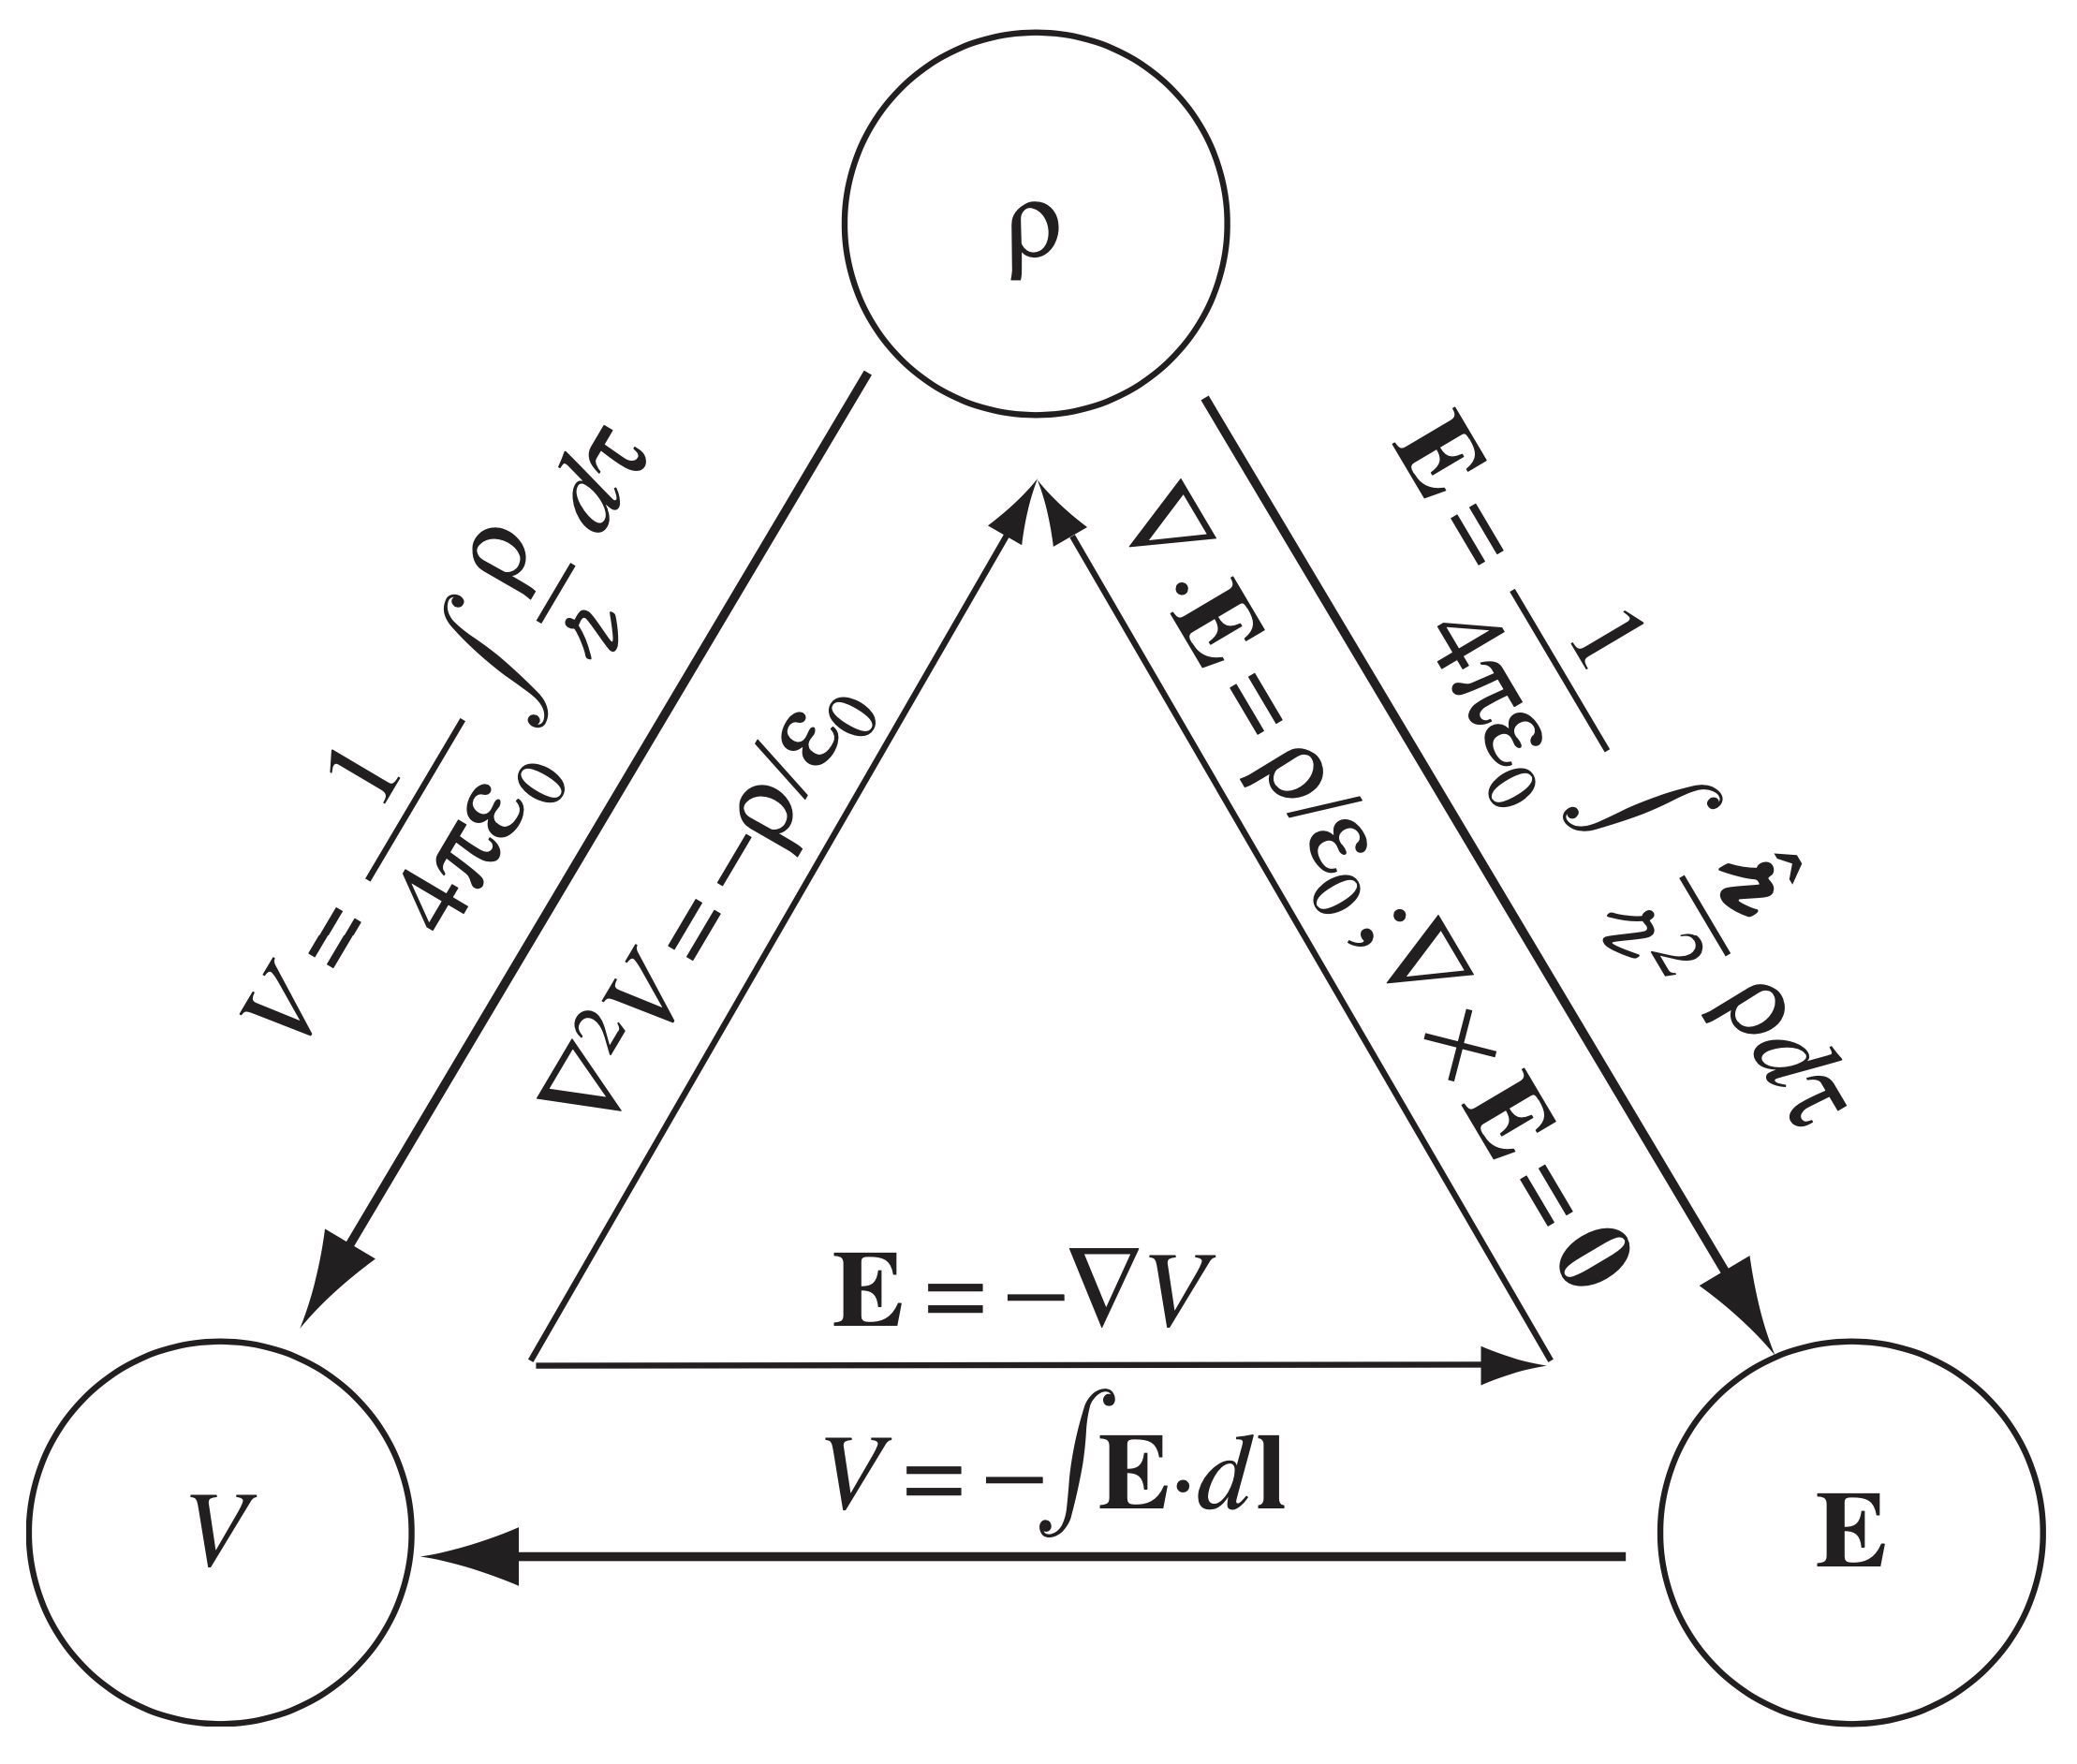
\includegraphics[scale=0.145]{em-triangle}
        \end{center}
    }
    
    \formbox{Other Notes}{
        \begin{itemize}
            \item For conductor problems, \textbf{always} check with
            Gauss's Law afterwards!
        \end{itemize}
    }
    
    \formula{Surface Field}{\vec{E}_\textrm{surf} = \frac{1}{2} \left( \vec{E}_\textrm{above} + \vec{E}_\textrm{below}\right)}
    
    \end{multicols*}

    \pagebreak


    \begin{multicols}{2}
        \formula{Generalized Multipole Expansion}{V(r) = \frac{1}{4\pi \epsilon_0}\sum_{n = 0}^\infty \frac{1}{r^{n + 1}} \int_{V} ||\vec{r'}||^n P_n(\cos \alpha)\rho(\vec{r'})d\tau'}
        \begin{multicols}{2}
            \formula{Monopole Voltage}{V(r) = \kfrac\frac{Q}{r}}
            \formula{Dipole Voltage}{V(r) = \kfrac \frac{\vec{p}\cdot \hat{r}}{r^2}}
        \end{multicols}
        \begin{multicols}{2}
            \formula{Dipole Moment -- Continuous Charge Distribution}{\vec{p} \equiv \int_V \vec{r'}\rho(\vec{r'})d\tau'   }
            \formula{Dipole Moment -- Change of Origin}{\vec{p'} = \vec{p} - Q\vec{a}}
            \formula{Torque of a Dipole}{\vec{N} = \vec{p} \times \vec{E}}
            \formula{Dipole Moment -- Point Charge Distribution}{\vec{p} = \sum_{i = 1}^n q_i \vec{r'}_i}
            \formula{Force on a Dipole}{\vec{F} = (\vec{p} \cdot \nabla)\vec{E}}
            \formula{Energy of a Dipole in an Electric Field}{U = -\vec{p} \cdot \vec{E}}
        \end{multicols}
        
        \begin{multicols}{2}
            \formula{Bound Surface Charge Density}{\sigma_\textrm{bound} = \vec{P} \cdot \hat{n}}
            \tripleformula{Linear Dielectrics}{\vec{P} &= \epsilon_0 \chi_e \vec{E}}{\vec{D} &= \epsilon \vec{E}}{\epsilon &= \epsilon_0 (1 + \chi_e) = \epsilon_0 \epsilon_r}
            \formula{Electric Displacement}{\vec{D} \equiv \epsilon_0 \vec{E} + \vec{P}}
            \formula{Displacement Boundary Condition}{D_\textrm{above}^\perp - D_\textrm{below}^\perp = \sigma_\textrm{free}}
            \formula{Image Charge Surface Charge}{\sigma = - \epsilon_0 \frac{\partial V}{\partial n}}
            \formula{Bound Volume Charge Density}{\rho_\textrm{bound} \equiv -\nabla \cdot \vec{P}}
            \doubleformula{Gauss's Law for Electric Displacement }{\nabla \cdot \vec{D} = \rho_f}{\oint\vec{D} \cdot d\vec{A} = Q_{f_\textrm{encl}}}
            \formula{Force on a Dielectric}{F = -\nabla U}
        \end{multicols}
        \formula{Solution for For Spherical Laplacians}{f(r, \theta) = \sum_{l = 0}^\infty{\left(A_l r^l + \frac{B_l}{r^{l + 1}}\right)P_l(\cos \theta)}}
        \begin{multicols}{2}
            \formbox{Legendre Polynomials}{\begin{align*}
                P_0(\cos \theta) &= 1\\
                P_1(\cos \theta) &= \cos\theta \\
                P_2(\cos \theta) &= \frac{3}{2} \cos^2 \theta - \frac{1}{2}\\
                P_3(\cos \theta) &= \frac{5}{2} \cos^3 \theta - \frac{3}{2} \cos \theta
            \end{align*}}
            
            \formula{Field of a Dipole}{\vec{E} = \kfrac\frac{p}{r^2}\left(2 \cos \theta \hat{r} + \sin \theta \hat{\theta}\right)}
            \formula{Work of a Dielectric}{W = \frac{1}{2}\int \vec{D} \cdot \vec{E} d\tau}
            \formbox{Names of Stuff}{
                $\epsilon_0$: Permittivity of Free Space\\
                $\epsilon_r$: Dielectric Constant or \\
                \hspace{0.5cm}Relative Permittivity\\
                $\epsilon$: Permittivity of a Material
            }
        \end{multicols}
        \vfill\null\columnbreak
        \formbox{Common Boundary Conditions}{
            \begin{itemize}
                \item $\vec{D}_\textrm{above}^\perp - \vec{D}_\textrm{below}^\perp = \sigma_f$
                \item $\vec{D}_\textrm{above}^\parallel - \vec{D}_\textrm{below}^\parallel = \vec{P}_\textrm{above}^\parallel - \vec{P}_\textrm{below}^\parallel$
                \item $\vec{E}_\textrm{above}^\perp - \vec{E}_\textrm{below}^\perp = \frac{\sigma_\textrm{surf}}{\epsilon_0}$
                \item $V_\textrm{above} = V_\textrm{below}$
                \item $\epsilon_\textrm{above}E_\textrm{above}^\perp - \epsilon_\textrm{below}E_\textrm{below}^\perp = -\sigma_f$
                \item $\epsilon_\textrm{above}\frac{\partial V_a}{\partial n}^\perp - \epsilon_\textrm{below}\frac{\partial V_b}{\partial n}^\perp = \sigma_f$
                \item $V(r = 0) = $ finite
                \item $V(r \to \infty) = $ finite or zero.
            \end{itemize}
        }
        \doubleformula{Method of Images Voltage}{V (r, \theta) = \kfrac\left(\frac{q_1}{||\vec{r}_{\textrm{sep}_1}||} + \frac{q_2}{||\vec{r}_{\textrm{sep}_2}||}\right)}{\frac{-q_1}{q_2} = \frac{||\vec{r}_{\textrm{sep}_1}||}{||\vec{r}_{\textrm{sep}_2}||}}
        \begin{multicols}{2}
            \formula{Binomial Expansion}{(1 + x)^k = \sum_{n = 0}^\infty{\left(\frac{k!}{n!(k - n)!}\right)}x^n}
        \end{multicols}
        \formbox{Takeaways from Practice}{
            \begin{itemize}
                \item Gauss's law inside a dielectric always includes both $\rho_b$ and $\sigma_b$.
                \item Use the definition for displacement where ever possible: $\vec{D} \equiv \epsilon_0 \vec{E} + \vec{P}$.
                \item The potential is constant below an image plane and the field is always zero. 
            \end{itemize}
        }
        \formula{Cylindrical Laplacian Solution}{
            V(s, \phi) = A \ln s + B + \sum_{n = 1}^\infty \left(A_n s^n + \frac{B_n}{s^n}\right) \left(C_n \cos (\phi n) + D_n \sin(\phi n)\right)
        }
        \formbox{General Problem Solving Strategy for Dielectrics}{
            \begin{enumerate}
                \item Check that your situation has irrotational displacement. Use $\nabla \times \vec{D} = 0$ or
                $\nabla \times \vec{P} = 0$. If your displacement is not irrotational, this is useless.
                \item If there are regions that have dielectrics, find the displacement using $\oint \vec{D} \cdot d\vec{A} = Q_\textrm{free, encl}$
                \item For regions without dielectrics, find the $\vec{E}$ field using Gauss's law.
                \item Using the results from (2) and (3), find $\vec{E}$ and $\vec{D}$ (whichever is lacking) 
                using principles of linear dielectrics.
                \item Use the definition of electric displacement to find $\vec{P}$: $\vec{D} \equiv \epsilon_0 \vec{E} + \vec{P}$.
            \end{enumerate}
        }
        \vfill\null
    \end{multicols}





\end{document}